\documentclass{article}
\usepackage{amsmath}
\usepackage{graphicx}

\begin{document}

\title{Box Membrane - Plane Wave Project}
\author{}
\date{\today}
\maketitle

\section{Introduction}
This document will track all steps in the development of the Box Membrane - Plane Wave project. The project consists of two main phases:
\begin{itemize}
    \item \textbf{Phase 1:} Setting up the numerical solutions for the wave equation on a stretched membrane.
    \item \textbf{Phase 2:} Using the numerical results to animate the interaction in Blender.
\end{itemize}

\section{Project Setup}
The project directory was created, and version control was initialized with Git. The project was then linked to a GitHub repository for remote access.

\section{Numerical Solution Setup}

We begin by defining the necessary parameters for simulating the wave equation on a rectangular membrane.

\subsection{Simulation Parameters}
The membrane dimensions are set to 1m by 1m, and the wave speed is chosen to be 1 m/s. The grid is discretized into 100 points along each dimension, resulting in a grid spacing of $\Delta x = \Delta y = 0.01$ m. We use a time step of $\Delta t = 0.001$ s for stability. 

\subsection{Initialization of Displacement Arrays}
Three displacement arrays are initialized:
\begin{itemize}
    \item $u$: Displacement at the current time step.
    \item $u_{\text{prev}}$: Displacement at the previous time step.
    \item $u_{\text{next}}$: Displacement at the next time step.
\end{itemize}

The initial conditions are set so that the membrane is at rest, with zero initial displacement and velocity.

\section{Numerical Solution of the Wave Equation}

To simulate the wave equation on a rectangular membrane, we use a finite difference time-stepping loop. The Courant-Friedrichs-Lewy (CFL) condition is applied to ensure stability, with $c \Delta t / \Delta x \leq 1$.

\subsection{Time-Stepping Loop}
The displacement at each grid point $(i, j)$ and time step $n+1$ is computed as:
\[
u_{i, j}^{n+1} = 2u_{i, j}^n - u_{i, j}^{n-1} + \text{CFL}^2 \left( \frac{u_{i+1, j}^n - 2u_{i, j}^n + u_{i-1, j}^n}{\Delta x^2} + \frac{u_{i, j+1}^n - 2u_{i, j}^n + u_{i, j-1}^n}{\Delta y^2} \right)
\]
where $\text{CFL} = \frac{c \Delta t}{\Delta x}$.

\subsection{Visualization}
To visualize the simulation, we plot the membrane's displacement every 100 time steps.

\begin{figure}[h!]
\centering
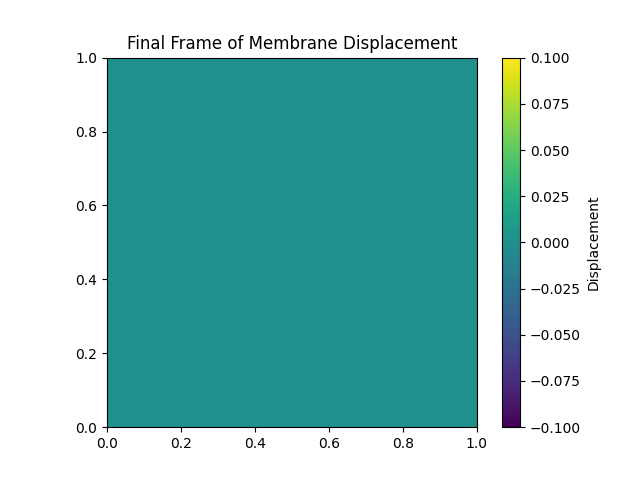
\includegraphics[width=0.7\textwidth]{simulation.png}
\caption{Sample visualization of the membrane's displacement.}
\end{figure}

\section{Dynamic Configurations for Enhanced Simulation}

To increase the dynamics of the membrane simulation, we introduced three configurable options in the code: a source term, an initial Gaussian pulse, and damping boundaries. Each option can be enabled or disabled through boolean variables, allowing for flexible testing and exploration of different behaviors.

\subsection{Configuration Options}

\begin{itemize}
    \item \textbf{Source Term:} A source term simulates an external sinusoidal disturbance at the center of the membrane. The source is defined by an amplitude $A$ and frequency $\omega$, with a sinusoidal input at each time step $n$:
    \[
    u_{\text{src}} = A \sin(\omega n \Delta t)
    \]
    where $A$ is the amplitude and $\omega = 2 \pi \times \text{freq}$, with $\text{freq}$ representing the desired frequency in Hz. This term introduces an ongoing interaction with the membrane, creating more dynamic behavior.

    \item \textbf{Gaussian Initial Condition:} Rather than starting the membrane at rest, we initialize it with a Gaussian-shaped displacement centered at $(x_0, y_0)$:
    \[
    u(x, y) = \exp\left(-\frac{(x - x_0)^2 + (y - y_0)^2}{2\sigma^2}\right)
    \]
    where $\sigma$ controls the spread of the initial pulse. This configuration leads to a spreading wave as the pulse propagates across the membrane.

    \item \textbf{Damping Boundaries:} To reduce reflections and simulate an infinite domain, damping is applied at the edges of the membrane grid. A damping factor $f$ (set to $0.9$) is applied to the boundary values of the displacement array $u_{\text{next}}$ at each time step:
    \[
    u_{\text{next}}[0, :], u_{\text{next}}[-1, :], u_{\text{next}}[:, 0], u_{\text{next}}[:, -1] \leftarrow f \times u_{\text{next}}[\text{boundary}]
    \]
    By gradually reducing displacement at the edges, the boundary damping minimizes wave reflections, allowing waves to dissipate as they would in an open space.
\end{itemize}

\subsection{Implementation in Python}

The code structure was modified to include boolean variables that control the activation of each configuration option:
\begin{verbatim}
use_source = True             # Enable or disable source term
use_gaussian_initial = True   # Enable or disable Gaussian initial condition
damping_boundaries = True     # Enable or disable damping at boundaries
\end{verbatim}

With these options, we can test different configurations by simply toggling the variables at the beginning of the code.

\subsection{Visualization and Output}

The simulation outputs an image file \texttt{simulation.png} representing the final frame of the membrane’s displacement. Additionally, the dynamics can be observed as a live plot, which updates every 100 time steps to visualize the changes over time.


\section{Enhanced Stability Adjustments}

To further stabilize the simulation, we implemented the following changes:

\subsection{Reduced Time Step}
The time step $\Delta t$ was reduced to $0.00025$ to better satisfy the Courant-Friedrichs-Lewy (CFL) condition and improve numerical stability.

\subsection{Domain-Wide Damping}
In addition to boundary damping, we applied a light damping factor across the entire domain to gradually dissipate energy and prevent excessive oscillations. This was controlled by an internal damping factor of 0.999, which slightly reduces the displacement values at each time step.

\subsection{Diagnostic Checks for Instability}
To monitor the simulation for potential instability, a diagnostic check was introduced to detect large displacements. If any displacement exceeds a threshold of $10^3$, a warning is triggered, and the simulation halts. This check helps identify divergence early in the time-stepping loop.

\section{Summary of Adjustments}

The following modifications were made to improve stability and prevent runtime errors:
\begin{itemize}
    \item Time step $\Delta t$ reduced to $0.00025$.
    \item Domain-wide light damping applied with a damping factor of 0.999.
    \item Diagnostic threshold set to monitor displacement values, triggering a warning if values exceed $10^3$.
\end{itemize}

These adjustments have stabilized the simulation and ensured that the wave propagates as expected without causing overflow or runtime errors.

\section{Final Adjustments and Animation Setup}

After stabilizing the simulation, the following adjustments were made to implement the animation and complete the simulation framework.

\subsection{Animation Setup}
The dynamics of the membrane were visualized by creating an animation. We used the \texttt{matplotlib.animation} module in Python to animate the simulation by updating the membrane’s displacement at each time step. The \texttt{FuncAnimation} class was employed to render each frame and update the membrane’s state over time.

The following settings were used for the animation:
\begin{itemize}
    \item \textbf{Frame Interval:} Each frame represents a single time step, with a delay of 20 ms per frame.
    \item \textbf{FPS (Frames Per Second):} We set 30 frames per second for a smooth visualization.
    \item \textbf{Output Format:} The animation was saved as a GIF file using the \texttt{Pillow} library due to the unavailability of \texttt{ffmpeg}.
\end{itemize}

\subsection{Summary of Final Stability Adjustments}
Several stability adjustments were applied to ensure that the simulation runs without errors:
\begin{itemize}
    \item \textbf{Reduced Time Step:} The time step $\Delta t$ was set to $0.00025$ to maintain stability according to the Courant-Friedrichs-Lewy (CFL) condition.
    \item \textbf{Domain-wide Damping:} A light damping factor of 0.999 was applied across the entire grid to reduce oscillations and energy accumulation within the membrane.
    \item \textbf{Boundary Damping:} Additional damping was applied along the boundaries of the membrane to simulate energy dissipation at the edges.
    \item \textbf{Diagnostic Check for Instability:} A diagnostic threshold was implemented to monitor displacement values and warn of potential instabilities if displacement exceeded a predefined threshold.
\end{itemize}

These adjustments enabled the creation of a stable and visually informative animation of the membrane dynamics.

\subsection{Conclusion}
This simulation provided a comprehensive visualization of membrane dynamics in response to initial conditions and optional external forces. The final setup, along with the animation, allows for further exploration of wave interactions on a two-dimensional surface. The code and documentation have been saved to a GitHub repository for version control and collaboration.

\section{Code and Repository Management}
All code and documentation files were committed to GitHub for version control. The final repository contains:
\begin{itemize}
    \item \texttt{simulation.py}: The main Python script for running the membrane simulation and generating the animation.
    \item \texttt{documentation.tex}: The LaTeX documentation file detailing the project steps, adjustments, and findings.
    \item \texttt{simulation.gif}: The final animation showing the dynamics of the membrane.
\end{itemize}


\end{document}
